\documentclass[]{beamer}
\usepackage[T1]{fontenc}
\usepackage[utf8]{inputenc}
\usepackage{lmodern}
\usepackage[italian]{babel}
\usepackage{mathrsfs}
\usepackage{cancel}
\usepackage{multicol}

\title{I numeri razionali}
\author{Mattia Cozzi}
\date{a.f.~2024/2025}
%\documentclass[handout]{beamer}     %usare questa classe per generare l'handout
%\usepackage{pgfpages}   %per mostrare più quadri nella stessa pagina
%\pgfpagesuselayout{4 on 1}[a4paper,border shrink=5mm,landscape]
\usetheme{Singapore}
%\useoutertheme[left]{sidebar} %elementi intorno alle diapositive
\setbeamercovered{dynamic} %modifica l'aspetto del testo grigetto delle diapositive future. Argomenti: invisible/transparent/dynamic

\usecolortheme{orchid}

%COLORE PRINCIPALE
\definecolor{verde}{RGB}{179, 0, 170} % UBC Blue (primary)
\setbeamercolor{structure}{fg=verde} % itemize, enumerate, etc
\setbeamercolor{alerted text}{fg=verde}


\theoremstyle{plain}
\newtheorem{teorema}{Teorema}

\usepackage{tikz}
\usepackage{circuitikz}

\usepackage{pgf,pgfplots,graphicx}
\usetikzlibrary{angles,quotes,arrows,shapes,decorations.markings}
\pgfplotsset{compat=1.15}
\usepgfplotslibrary{units,fillbetween} % to add units easily to axis


\def\angolo[#1](#2)(#3:#4:#5)% Syntax: [draw options] (center) (initial angle:final angle:radius)
    { \draw[#1] ($(#2)+({#5*cos(#3)},{#5*sin(#3)})$) arc (#3:#4:#5); }


\begin{document}

\begin{frame}
  \titlepage
\end{frame}





\begin{frame}
\frametitle{Contenuti}
\tableofcontents
\end{frame}


\section{Divisibilità}

\begin{frame}
\frametitle{Divisibilità}
Dati due numeri interi, è possibile che:

~
\begin{itemize}
  \item la divisione tra loro sia esatta, senza resto, come in:
  \begin{center}$ 12 : 3 = 4$, resto $0$\end{center}
  Diciamo allora che il primo numero \alert{è divisibile} per il secondo.\pause

  ~
  \item  la divisione tra loro abbia resto, come in:
  \begin{center}$ 13 : 3 = 4$, resto $1$\end{center}
  Diciamo allora che il primo numero \alert{non è divisibile} per il secondo.
\end{itemize}
\end{frame}


\begin{frame}
\frametitle{Multipli e sottomultipli/divisori}
Se il numero $a$ è divisibile per il numero $b$, allora:

~
\begin{itemize}
  \item $a$ è \alert{multiplo} di $b$;
  \begin{center}$21$ è multiplo di $7$\end{center}\pause
  
  ~
  \item $b$ è \alert{sottomultiplo o divisore} di $a$.
  \item \begin{center}$7$ è sottomultiplo di $21$\end{center}
\end{itemize}
\end{frame}


\begin{frame}
\frametitle{Una conseguenza}
Se il prodotto di due numeri dà come risultato un terzo numero, allora quest'ultimo è multiplo degli altri due.\pause

~

\[5 \cdot 9 = 45 \]
Quindi 45 è multiplo sia di 5, sia di 9.
\end{frame}


\begin{frame}
\frametitle{E i numeri negativi?}
Lo stesso discorso, senza variazioni, vale coi numeri negativi:
\begin{center}
  $ -63 : 7 = -9 $
\end{center}\pause
e quindi:
\begin{itemize}
  \item $ -63 $ è multiplo di $ 7 $ e di $ -9 $;\pause
  \item $ 7 $ e $ -9 $ sono divisori di $ - 63 $.\pause
\end{itemize}

~

Ti ricordi la \alert{regola dei segni}?
\end{frame}


\begin{frame}
\frametitle{Domande interessanti}
\begin{itemize}
  \item Qual è il numero che è multiplo di tutti i numeri interi?\pause
  
  ~

  \item Qual è il numero che è sottomultiplo di tutti i numeri interi?
\end{itemize}
\end{frame}


\begin{frame}
\frametitle{Pari e dispari in $\mathbb{N}$}
I \alert{numeri pari} sono i multipli di 2, e quindi terminano con:
\begin{center}
  0, 2, 4, 6, 8
\end{center}\pause
Sono indicati con:
\[ \mathbb{P} = \{ 0, 2, 4, 6, 8, 10, 12, \ldots \} \]\pause

~

I \alert{numeri dispari} sono i numeri che non sono pari, e quindi terminano con:
\begin{center}
  1, 3, 5, 7, 9
\end{center}\pause
\[ \mathbb{D} = \{ 1, 3, 5, 7, 9, 11, 13, \ldots \} \]
\end{frame}


\begin{frame}
\frametitle{Pari e dispari in $\mathbb{Z}$}
Il concetto di pari e dispari si estende anche ai numeri interi (positivi e negativi:)
\[ \mathbb{P} = \{ \ldots, -6, -4, -2, 0, +2, +4, +6, \ldots \} \]\pause

\[ \mathbb{D} = \{ \ldots, -5, -3, -1, 0, +1, +3, +5, \ldots \} \]\pause
\end{frame}


\section{Criteri}

\begin{frame}
\frametitle{Criteri di divisibilità}
I criteri di divisibilità sono dei \alert{criteri} per capire se un numero intero è divisibile per un altro, senza calcolare per davvero la divisione.\pause

~

Potremo ad esempio rispondere, senza far calcoli, alle seguenti domande:
\begin{itemize}
  \item 1404 è divisibile per 9?\pause
  \item 153 è divisibile per 11?
\end{itemize}
\end{frame}


\begin{frame}
\frametitle{Divisibilità per 2}
\begin{block}{Critero di divisibilità per 2}
  Un numero è divisibile per 2 se è pari, cioè se finisce per:
  \begin{center}
    0, 2, 4, 6, 8
  \end{center}
\end{block}\pause

~

\begin{itemize}
  \item 487238 è divisibile per 2;\pause
  \item 400 è divisibile per 2.
\end{itemize}
\end{frame}



\begin{frame}
\frametitle{Divisibilità per 3}
\begin{block}{Critero di divisibilità per 3}
  Un numero è divisibile per 3 se la somma delle sue cifre è un multiplo di 3.
\end{block}\pause

~

\begin{itemize}
  \item 171 è divisibile per 3, perché $ 1+ 7+ 1 = 9 $;\pause
  \item 3477 è divisibile per 3, perché $ 3 + 4+ 7+ 7 = 21 $.
\end{itemize}
\end{frame}


\begin{frame}
\frametitle{Divisibilità per 6}
\begin{block}{Critero di divisibilità per 6}
  Un numero è divisibile per 6 se è divisibile sia, per 2 sia per 3.
\end{block}\pause

~

\begin{itemize}
  \item 492 è divisibile per 6, perché è pari e $ 4 + 9 + 2 = 15 $.
\end{itemize}
\end{frame}


\begin{frame}
\frametitle{Divisibilità per 5}
\begin{block}{Critero di divisibilità per 5}
  Un numero è divisibile per 5 se finisce con 0 oppure 5.
\end{block}\pause

~

\begin{itemize}
  \item 4565 è divisibile per 5;\pause
  \item 150 è divisibile per 5.
\end{itemize}
\end{frame}


\begin{frame}
\frametitle{Divisibilità per 9}
\begin{block}{Critero di divisibilità per 9}
  Un numero è divisibile per 9 se la somma delle sue cifre è un multiplo di 9.

  ~

  Prova a considerare la tabellina del 9!
\end{block}\pause

~

\begin{itemize}
  \item 171 è divisibile per 9, perché $ 1+ 7+ 1 = 9 $;\pause
  \item 48672 è divisibile per 9, perché $ 4 + 8+6+ 7+ 2 = 27 $.
\end{itemize}
\end{frame}


\begin{frame}
\frametitle{Divisibilità per 10}
\begin{block}{Critero di divisibilità per 10}
  Un numero è divisibile per 10 se finisce per 0.
\end{block}\pause

~

\begin{itemize}
  \item 1360 è divisibile per 10.
\end{itemize}
\end{frame}


\begin{frame}
\frametitle{Divisibilità per 7}
\begin{block}{Critero di divisibilità per 7}
  Un numero è divisibile per 7 se la differenza tra le decine e il doppio delle unità è un multiplo di 7.
\end{block}\pause

~

\begin{itemize}
  \item 91 è divisibile per 7, perché $ 9- 1 \cdot 2 = 7 $;\pause
  \item 231 è divisibile per 7, perché $ 23 - 1 \cdot 2 = 21 $.
\end{itemize}
\end{frame}




\begin{frame}
\frametitle{Divisibilità per 11}
\begin{block}{Critero di divisibilità per 11}
  Un numero è divisibile per 11 se la differenza tra la somma delle cifre di posto dispari e quella delle cifre di posto pari è un multiplo di 11.
\end{block}\pause

~

\begin{itemize}
  \item 121 è divisibile per 11, perché $ (1+1) - (2) = 0 $;\pause
  \item 9273 è divisibile per 11, perché $ (9+7) - (2+3) = 11 $.
\end{itemize}
  

\end{frame}




\begin{frame}
\frametitle{Divisibilità per 4}
\frametitle{Divisibilità per 4}
\begin{block}{Critero di divisibilità per 4}
  Un numero è divisibile per 4 se le ultime due cifre sono un multiplo di 4.
\end{block}\pause

~

\begin{itemize}
  \item 412 è multiplo di 4;\pause
  \item 576 è multiplo di 4.
\end{itemize}
\end{frame}




\section{Primi}



\begin{frame}
\frametitle{Numeri primi}
I numeri primi sono tutti e soli i numeri naturali che sono \alert{divisibili soltanto per 1 e per sé stessi}.\pause

~

7 è un numero primo, perché può essere diviso solo per 1 e per 7.\pause

~

I numeri non primi si dicono composti, come 12 (divisibile per un sacco di numeri!).\pause

~

1 non viene considerato un numero primo.\pause

~

I numeri primi sono \alert{infiniti}!
\end{frame}


\begin{frame}
\frametitle{Numeri primi da 1 a 50}
\begin{table}[]
  \begin{tabular}{ccccc}
  ~~~~2~~~~  & ~~~~3~~~~  & ~~~~5~~~~  & ~~~~7~~~~  & ~~~~11~~~~ \\
  &&&& \\
  13 & 17 & 19 & 23 & 29 \\
  &&&& \\
  31 & 37 & 41 & 43 & 47                    
  \end{tabular}
  \end{table}
\end{frame}





\begin{frame}
\frametitle{Scomposizione in fattori primi}
È stato dimostrato che:
\begin{center}
  \alert{ogni numero naturale può essere scritto come prodotto di soli numeri primi.}
\end{center}\pause

~

Ad esempio:\[ 153 = 3 \cdot 3 \cdot 17 \]\pause\[ 385 = 5 \cdot 7 \cdot 11 \]\pause
Questo procedimento è detto \alert{scomposizione o fattorizzazione} in numeri primi.
\end{frame}


\begin{frame}
\frametitle{Esempio di scomposizione}
Proviamo a scomporre 180 in fattori primi:
\begin{table}[]
  \begin{tabular}{r|l}
  180\pause\pause & 2\pause \\
  90 \pause & 2\pause \\
  45 \pause & 3\pause \\
  15 \pause & 3\pause \\
  5  \pause & 5\pause \\
  1   &  
  \end{tabular}\pause

  ~

  Possiamo scrivere la fattorizzazione di 180:
  \[ 180 = 2 \cdot 2 \cdot 3 \cdot 3 \cdot 5 \pause= 2^2 \cdot 3^2 \cdot 5 \]
  \end{table}
\end{frame}


\begin{frame}
\frametitle{Esercizi sulla scomposizione in fattori primi}
\begin{enumerate}
  \item Scomponi in fattori primi i seguenti numeri:
  \begin{multicols}{2}
    \begin{itemize}
        \item $ 152 $
        \item $ 90 $
        \item $ 156 $
        \item $ 612 $
        \item $ 720 $
        \item $ 1024 $
    \end{itemize}
  \end{multicols}
\end{enumerate}
\end{frame}


\begin{frame}
\frametitle{Massimo comun divisore (MCD)}
Il massimo comun divisore (indicato con MCD) tra due numeri è \alert{il più alto dei divisori comuni tra due numeri}.\pause

~

Elenchiamo i divisori di 24:
\[div(24) = \{ 1, 2, 3, 4, 6, 8, \alert<3->{12}, 24 \}\]\pause

Elenchiamo i divisori di 36:
\[div(36) = \{ 1, 2, 3, 4, 6, 9, \alert<3->{12}, 18, 36 \}\]\pause

Quindi il massimo comun divisore tra 24 e 36 è 12.\pause

~

Esiste un modo più veloce per calcolare l'MCD tra due numeri?
\end{frame}

\begin{frame}
\frametitle{Calcolo dell'MCD}
Eseguo le seguenti operazioni:

~

\begin{enumerate}
  \item \alert{scompongo in fattori primi} i due numeri;\pause
  
  ~
  \item costruisco l'MCD scegliendo, nelle scomposizioni, \alert{i fattori in comune, con l'esponente più basso}.\pause
\end{enumerate}

~

Esempio:\[24 = 2^3 \cdot \alert<4->{3} \qquad\qquad 36 = \alert<4->{2^2} \cdot 3^2 \]\pause

\[ MCD(24, 36) = \alert<4->{2^2} \cdot \alert<4->{3} \]
\end{frame}







\begin{frame}
  \frametitle{Esercizi sull'MCD}
  \begin{enumerate}
    \item Calcola il Massimo Comun Divisore fra i seguenti gruppi di numeri.
    \begin{multicols}{2}
      \begin{itemize}
          \item $ 18, 96 $
          \item $ 9, 108 $
          \item $ 26, 64 $
          \item $ 3, 7, 9 $
          \item $ 14, 35, 21 $
          \item $ 36, 108, 117 $
      \end{itemize}
    \end{multicols}
  \end{enumerate}
  \end{frame}
  
  





\begin{frame}
\frametitle{Minimo comune multiplo (mcm)}
Il minimo comune multiplo (indicato con mcm) tra due numeri è \alert{il più piccolo tra i multipli comuni tra due numeri} diverso da zero.\pause

~

Elenchiamo i multipli di 6:
\[mult(6) = \{ 0, 6, 12, 18, 24, \alert<3->{30}, 36, 42, 48, 54, 60, \ldots \}\]\pause

Elenchiamo i multipli di 15:
\[mult(15) = \{ 0, 15, \alert<3->{30}, 45, 60, 75, 90, \ldots \}\]\pause

Quindi il minimo comun divisore tra 6 e 15 è 30.\pause

~

Esiste un modo più veloce per calcolare l'mcm tra due numeri?
\end{frame}


\begin{frame}
\frametitle{Calcolo dell'mcm}
Eseguo le seguenti operazioni:

~

\begin{enumerate}
  \item \alert{scompongo in fattori primi} i due numeri;\pause
  
  ~
  \item costruisco l'mcm scegliendo, nelle scomposizioni, \alert{tutti i fattori (comuni e non comuni), con l'esponente più alto}.\pause
\end{enumerate}

~

Esempio:\[24 = \alert<4->{2^3} \cdot \alert<4->{3} \qquad\qquad 28 = 2^2 \cdot \alert<4->{7} \]\pause

\[ mcm(24, 28) = \alert<4->{2^3} \cdot \alert<4->{3} \cdot \alert<4->{7} \]
\end{frame}




\begin{frame}
\frametitle{Esercizi sull'mcm}
\begin{enumerate}
    \item Calcola il minimo comune multiplo fra i seguenti gruppi di numeri.
    \begin{multicols}{2}
      \begin{itemize}
          \item $ 18, 96 $
          \item $ 9, 108 $
          \item $ 26, 64 $
          \item $ 3, 7, 9 $
          \item $ 14, 35, 21 $
          \item $ 36, 108, 117 $
      \end{itemize}
    \end{multicols}
    \item In un campanile ci sono tre campane. Una batte un rintocco ogni 5 secondi, la seconda un rintocco ogni 6 secondi, la terza batte un rintocco ogni 8 secondi. Se battono insieme il primo rintocco, dopo quanti secondi ne batteranno un altro insieme?
\end{enumerate}
\end{frame}
  



\section{Frazioni}

\begin{frame}
\frametitle{Perché le frazioni?}
I numeri decimali e i numeri interi, sia positivi sia negativi, possono essere anche espressi sotto forma di \alert{frazioni}, che vanno a costituire l'insieme $ \mathbb{Q} $ dei \alert{numeri razionali}.\pause

~

Ad esempio:
\begin{center}
  $ 7,7 = 77 : 10 = \dfrac{77}{10} $\pause
  
  ~

  ~

  $ -2,3 = -23 : 10 = -\dfrac{23}{10} $
\end{center}\pause

Le frazioni sono solo un modo più comodo di scrivere delle divisioni!
\end{frame}




\begin{frame}
\frametitle{L'insieme $ \mathbb{Q} $}
Le frazioni, cioè i numeri decimali (finiti oppure periodici), costituiscono l'insieme $ \mathbb{Q} $, cioè l'insieme dei \alert{numeri razionali} (\emph{ratio} in latino significa ``rapporto'', cioè divisione.)
  
\begin{figure}
  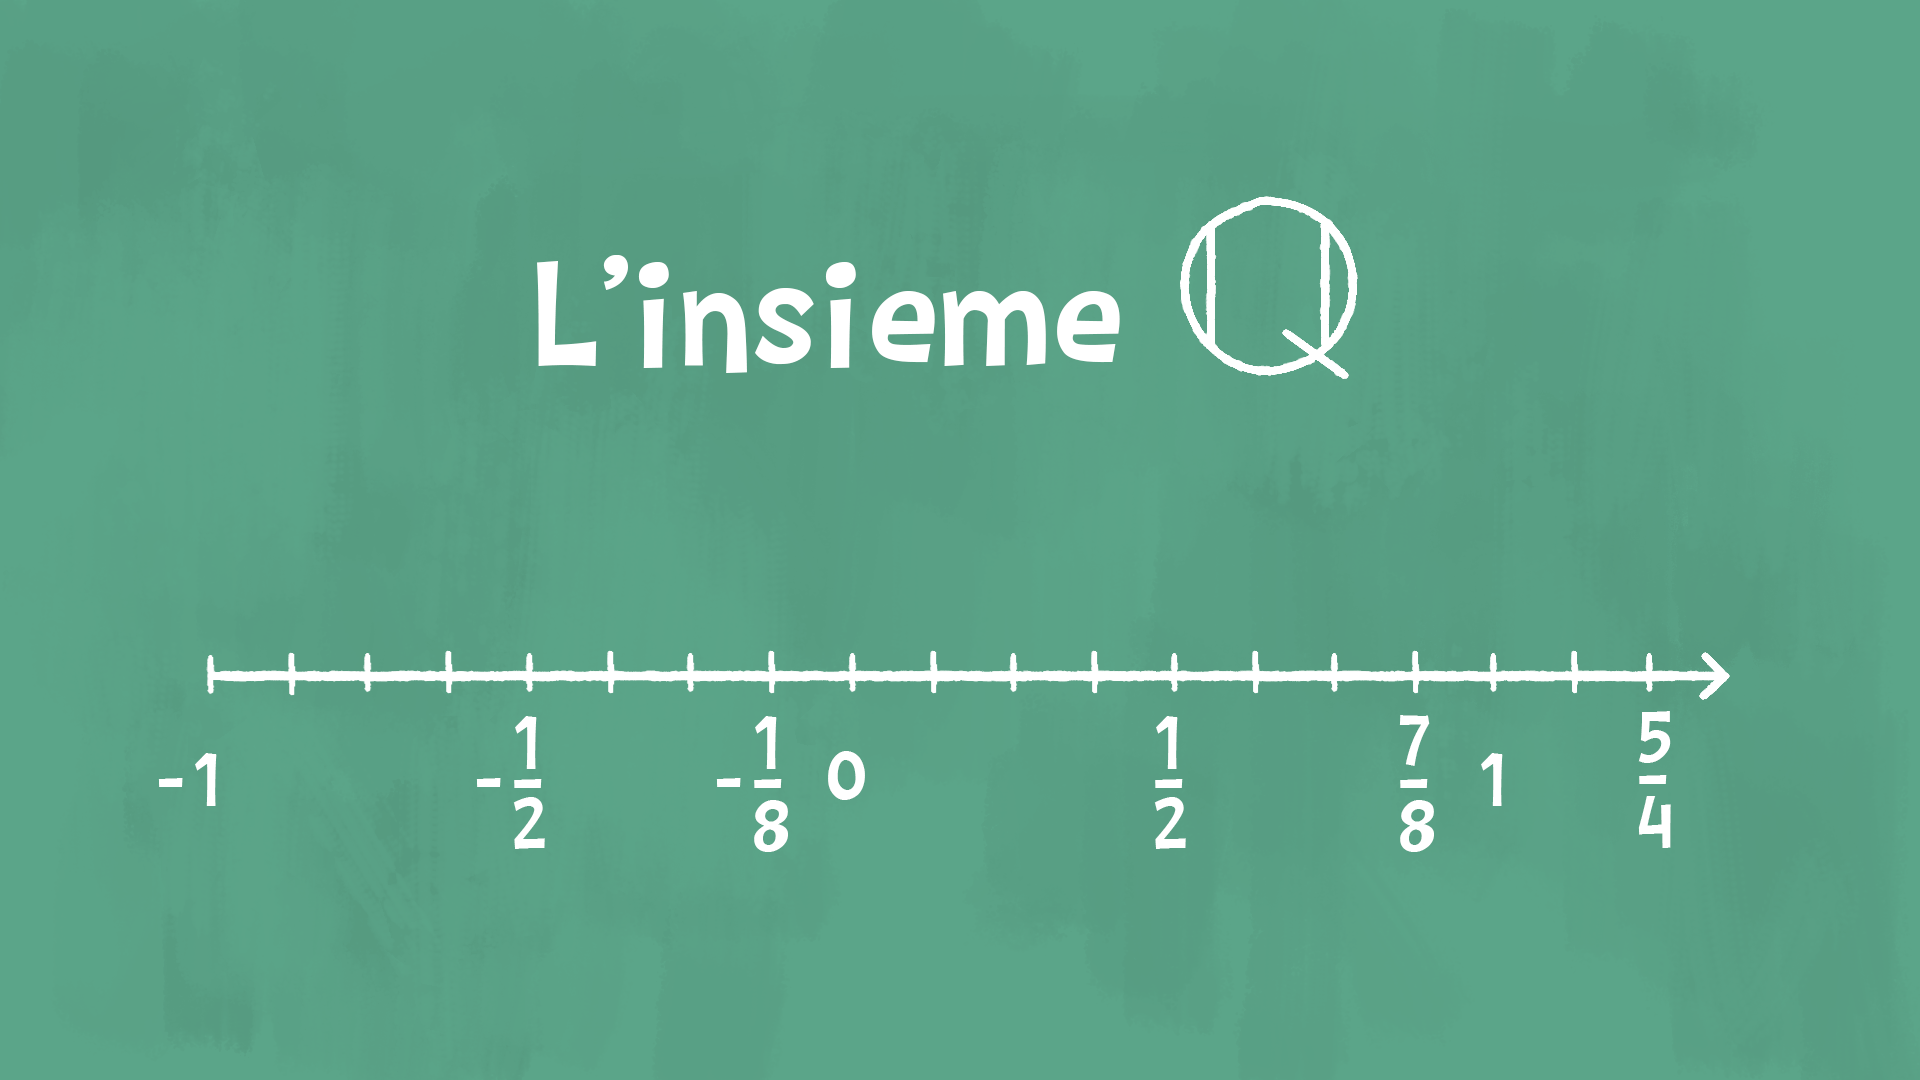
\includegraphics[width=.65\columnwidth]{img/rettaq.png}
\end{figure}\pause

Stiamo riempiendo lo spazio tra un numero e l'altro che c'era in $ \mathbb{Z} $.
\end{frame}




\begin{frame}
\frametitle{Insiemi numerici}

\begin{figure}
  \begin{tikzpicture}
    \draw[thick, purple] (0,0) ellipse (3cm and 1.5cm);
    \node[purple] at (2,.4) {$ \mathbb{N} $};
    \node[below,purple] at (2,.4) {naturali};
    \node[] at (-2,0) {$ 2 $};
    \node[] at (0,1) {$ 10 $};
    \node[] at (1,-1) {$ 135 $};
    \draw[thick, blue] (.6,0) ellipse (4cm and 2.5cm);
    \node[blue] at (3.8,.4) {$ \mathbb{Z} $};
    \node[below,blue] at (3.8,.4) {interi};
    \node[] at (2.5,1.3) {$ -6 $};
    \node[] at (1,-1.8) {$ -1 $};
    \node[] at (1,1.8) {$ -100 $};
    \draw[thick, red] (1.2,0) ellipse (5cm and 3.5cm);
    \node[red] at (5.4,.4) {$ \mathbb{Q} $};
    \node[below,red] at (5.4,.4) {razionali};
    \node[] at (4.5,1.7) {$ \dfrac{2}{3} $};
    \node[] at (4.5,-1.7) {$ -\dfrac{23}{10} $};
    \node[] at (3,-2.7) {$ \dfrac{16}{7} $};
\end{tikzpicture}
\end{figure}
\end{frame}




\begin{frame}
\frametitle{Cosa resta fuori}
L'insieme $ \mathbb{Q} $ non esaurisce l'insieme dei numeri che si usano in matematica.\pause

~

La sua estensione è l'insieme $ \mathbb{R} $ dei \alert{numeri reali}.\pause

~

$ \mathbb{R} $ contiene numeri decimali non periodici, cioè con un numero infinito di cifre casuali dopo la virgola, che non si ripetono mai.\pause

~

Qualche esempio di numero reale ma non razionale:
\begin{center}
  $ \pi = 3,141592653589\ldots $

  ~

  $ \sqrt{2} = 1,4142135623730\ldots $
\end{center}
\end{frame}




\begin{frame}
\frametitle{Insiemi numerici}
\begin{figure}
  \begin{tikzpicture}[scale=.8]
    \draw[thick, purple] (0,0) ellipse (3cm and 1.5cm);
    \node[purple] at (2,.4) {$ \mathbb{N} $};
    \node[] at (-2,0) {$ 2 $};
    \node[] at (0,1) {$ 10 $};
    \node[] at (1,-1) {$ 135 $};
    \draw[thick, blue] (.6,0) ellipse (4cm and 2.5cm);
    \node[blue] at (3.8,.4) {$ \mathbb{Z} $};
    \node[] at (2.5,1.3) {$ -6 $};
    \node[] at (1,-1.8) {$ -1 $};
    \node[] at (1,1.8) {$ -100 $};
    \draw[thick, red] (1.2,0) ellipse (5cm and 3.5cm);
    \node[red] at (5.4,.4) {$ \mathbb{Q} $};
    \node[] at (4.5,1.7) {$ \dfrac{2}{3} $};
    \node[] at (4.5,-1.7) {$ -\dfrac{23}{10} $};
    \node[] at (3,-2.7) {$ \dfrac{16}{7} $};
    \draw[thick, orange] (1.8,0) ellipse (6cm and 4.5cm);
    \node[orange] at (7.1,.4) {$ \mathbb{R} $};
    \node[] at (6.5,1.7) {$ \pi $};
    \node[] at (6.5,-1.7) {$ \sqrt{2} $};
    \node[] at (4,-3.7) {$ \sqrt{3} $};
\end{tikzpicture}
\end{figure}
\end{frame}







\begin{frame}
\frametitle{Terminologia}
Essendo le frazioni delle divisioni, possiamo introdurre dei nuovi termini:

~

\begin{itemize}
  \item il \alert{numeratore} è ``il numero sopra'', cioè il dividendo;\pause
  
  ~
  \item il \alert{denominatore} è il ``numero sotto'', cioè il divisore.\pause
\end{itemize}

~

~
\[\frac{15}{7}\]\pause
15 è il numeratore, 7 è il denominatore.
\end{frame}





\begin{frame}
\frametitle{Il valore di una frazione}
A volte, per capire bene il valore di un numero razionale (una frazione) è utile \alert{eseguire la divisione tra i due numeri}:
\[\frac{3}{8}=0,375\]\pause

Alcune frazioni, anche se in apparenza diverse, hanno in realtà \alert{lo stesso valore}:
\[\frac{3}{8}=\frac{9}{24}\]\pause
Quando due frazioni hanno lo stesso valore, si dicono \alert{frazioni equivalenti}.
  

\end{frame}



\begin{frame}
\frametitle{Minimi termini}
Per trovare la frazione \alert{più semplice} equivalente ad una certa frazione, si ricorre alla \alert{semplificazione}.\pause

~

Quando una frazione è espressa nella sua forma più semplice, si dice che è \alert{ridotta ai minimi termini}.

\begin{center}
  $ \dfrac{9}{24} $ \alert{non} è ridotta ai minimi termini


  ~

  ~

  $ \dfrac{3}{8} $ è ridotta ai minimi termini
\end{center}\pause

~

Per eseguire la semplificazione, è importantissimo essere abili nella \alert{scomposizione in fattori primi}.
\end{frame}

\begin{frame}
\frametitle{Semplificazione}
Possiamo semplificare una frazione \alert{dividendo numeratore e denominatore} per un fattore comune (il migliore è l'mcm, ma possiamo anche procedere per passi).\pause

~

Esempi:
\[ \frac{16}{10}\pause = \frac{8 \cdot 2}{5 \cdot 2}\pause = \frac{8 \cdot \cancel{2}}{5 \cdot \cancel{2}}\pause = \frac{8}{5} \]\pause

\[ \frac{14}{21}\pause = \frac{7 \cdot 2}{7 \cdot 3}\pause = \frac{\cancel{7}\cdot 2}{\cancel{7} \cdot 3}\pause = \frac{2}{3} \]
\end{frame}




\begin{frame}
  \frametitle{Esercizi sulla semplificazione delle frazioni}
  \begin{enumerate}
    \item Riduci ai minimi termini le seguenti frazioni:
    \begin{multicols}{2}
      \begin{itemize}
          \item $ \dfrac{4}{8} $
          
          ~

          ~
          \item $ \dfrac{10}{15} $
          
          ~

          ~
          \item $ \dfrac{100}{200} $
          \item $ \dfrac{16}{24} $
          
          ~

          ~
          \item $ \dfrac{2000}{3000} $
          
          ~

          ~
          \item $ \dfrac{8}{4} $
      \end{itemize}
    \end{multicols}
  \end{enumerate}
  \end{frame}
  


\begin{frame}
\frametitle{Rappresentare una frazione}
Per eseguire i calcoli con le frazioni, è molto utile \alert{immaginarle}, cioè vederle con l'immaginazione:

~
\begin{figure}
  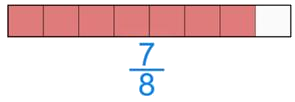
\includegraphics[width=.5\columnwidth]{img/fraz.png}
\end{figure}

La frazione rappresentata significa ``sette parti su otto'' (quindi meno di un intero, cioè 1).\pause

~

Prova a rappresentare $ \dfrac{7}{4} $. \pause

~

Cosa succede se il numeratore è maggiore del denominatore?
\end{frame}


\begin{frame}
\frametitle{Frazioni proprie, improprie e apparenti}
\begin{itemize}
  \item \alert{Frazioni proprie}, in cui il numeratore è più piccolo del denominatore (valgono quindi \alert{meno di 1});
  \[\frac{2}{3}=0,666\ldots\qquad\qquad\qquad\frac{99}{100}=0,99\]\pause
  \item \alert{frazioni apparenti}, in cui il numeratore è un multiplo del denominatore (equivalgono quindi a \alert{un numero intero});
  \[\frac{10}{5}=\frac{2}{1}=2\qquad\qquad\qquad\frac{40}{4}=\frac{10}{1}=10\]\pause
  \item \alert{frazioni improprie}, in cui il numeratore è un più grande del denominatore (valgono quindi \alert{più di 1});
  \[\frac{11}{5}=2,2\qquad\qquad\qquad\frac{13}{8}=1,625\]
\end{itemize}
  

\end{frame}


\begin{frame}
  \frametitle{Esercizi sulla rappresentazione delle frazioni}
  \begin{enumerate}
    \item Rappresenta le seguenti frazioni (se necessario, semplificale prima di disegnarle):
    \begin{multicols}{2}
      \begin{itemize}
          \item $ \dfrac{2}{5} $
          
          ~

          ~
          \item $ \dfrac{1}{9} $
          
          ~

          ~
          \item $ \dfrac{6}{12} $
          \item $ \dfrac{6}{5} $
          
          ~

          ~
          \item $ \dfrac{9}{3} $
          
          ~

          ~
          \item $ \dfrac{38}{19} $
      \end{itemize}
    \end{multicols}
    \item Scrivi 6 frazioni (2 proprie, 2 improprie e 2 apparenti) e rappresentale.
  \end{enumerate}
  \end{frame}
  




\section{Operazioni}


\begin{frame}
\frametitle{Frazioni ``compatibili''}
È molto facile eseguire la somma/differenza di frazioni quando queste hanno \alert{lo stesso denominatore}: basta sommare/sottrarre i numeratori:

~

\begin{figure}
  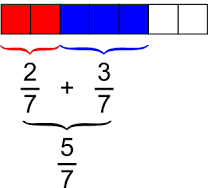
\includegraphics[width=.4\columnwidth]{img/sommafraz.png}
\end{figure}
\end{frame}


\begin{frame}
\frametitle{Esempi}
\[ \frac{3}{4} + \frac{7}{4} \pause= \frac{3+7}{4}\pause = \frac{10}{4}\pause = \frac{5}{2}  \]\pause

~

\[ \frac{7}{8} - \frac{5}{8} \pause= \frac{7-5}{8}\pause = \frac{2}{8}\pause = \frac{1}{4}  \]\pause

~

Come si esegue invece questo calcolo?
\[ \frac{2}{7} + \frac{3}{4} \]
\end{frame}



\section{Proporzioni}



\section{Percentuali}


\end{document}
r